\chapter{Introduction}
\label{sec:introduction}

Twenty years ago, Lieberman 
%described debugging as "the dirty little secret of computer science".
%He 
argued that the huge economic cost created by software bugs, resulting from the efforts to locate and fix bugs and the damages caused by bugs  not found in time, was not adequately matched by efforts to provide better debugging tools and establish better debugging practices.
Lieberman called this the "Debugging Scandal"~\cite{lieberman97:the_debugging_scandal}.
In his famous article, he urged the computer science community to stop ignoring this problem and outlines several directions in which debugging can be evolved.
Twenty years later, computer science research has produced many new and advanced approaches to debugging; in practice, however, the situation has barely improved~\cite{yin11:debugging_scandal_the_next, perscheid17:studying_the_advancement}.

\section{The Real Cost of Software Errors}

The amount of software that is involved in almost every aspect of our modern life is steadily increasing.
In many fields, including traditional engineering fields such as automotive engineering, innovation is largely driven by software these days~\cite{evans08:invisible_engines_how_software, gorschek10:a_lightweight_innovation_process}.
With the rise of cloud computing and devices becoming smarter and smarter, this trend will not stop in the near future.

%Software faults affect the operation of all professional and commercial software products and have been studied in many kinds of applications, such as web-browser~\cite{li06:have_things_changed_now}, enterprise applications~\cite{turhan09:data_mining_source_code, sahoo10:an_empirical_study}, and operating systems~\cite{guo10:characterizing_and_predicting_which}. % check sources
% In Mozilla's Firefox browser, 85\% of bugs were caused by incorrect implementations of requirements~\cite{li06:have_things_changed_now}.

It has long been recognized that there is no such thing as a bug-free program~\cite{schwartz71:an_overview_of_bugs}.
Software faults affect the operation of all professional and commercial software products.
%from web-browsers, over servers, to operating systems~\cite{li06:have_things_changed_now, sahoo10:an_empirical_study, guo10:characterizing_and_predicting_which}.
In 2002, the yearly economic cost of software errors was estimated to be above 60~billion dollars in the United States alone~\cite{tassey02:the_economic_impacts}. 
These damages are accumulated from a variety of sources.
Most obviously, errors need to be fixed and therefore increase the software development costs.
However, before developers can even begin to work on a fix, the errors have to be reproduced, classified, and prioritized; all activities that cost time and resources~\cite{sahoo10:an_empirical_study, guo10:characterizing_and_predicting_which}.

Further damages are incurred when the increased workload delays the project's release, as the increased time to market can lead to lost opportunities.
Usually, errors are most expensive when they manifest in production.
Not only can they cause direct costs by interrupting business operations, they are also more expensive to repair and can cause long-term damage through loss of reputation and future business for the company.
Additional billions of damage are created by failing software projects, where bugs are often part of the problem~\cite{charette05:why_software_fails, zhivich09:the_real_cost}. \todo{move zhivich}

%Finally, it is not only the economic damage that is worrisome.
%When software failures occur in critical infrastructure, lives are endangered.
%While total numbers are difficult to determine, there are many reports of incidents where faulty software systems were at least partially responsible for loss of human life~\cite{zhivich09:the_real_cost}.
%\todo{section divider}

\medskip\medskip\noindent
The majority of bugs in modern software systems are semantic bugs, \ie bugs where the code does not implement the intended behavior~\cite{li06:have_things_changed_now}.
Compared to memory or concurrency bugs, semantic bugs are notoriously hard to formalize and detect automatically.

%  between 25\% and
Accordingly, studies found that developers spend up to 60\% of their time on software bugs, debugging, and maintenance related activities~\cite{ballou08:improving_software_quality, hailpern02:software_debugging_testing, beizer03:software_testing_techniques}.
However, effective debugging skills are not only important to reduce development time.
An incorrect bug fix might not cover all corner cases or cause unexpected side-effects, thereby causing additional problems in the future.
In the Apache bug database, 9\% of bug reports were reopened due to bad fixes~\cite{gu10:has_the_bug_really}.
This number does not even include bad fixes for which a new bug report was created.
In a commercial operating system, between 15\% and 24\% of fixes for post-release bugs found were found incorrect and caused additional problems to users; for concurrency bugs, 39\% of fixes were faulty~\cite{yin11:how_do_fixes_become}.

Considering the total cost created by bugs in software, we would expect companies to encourage software developers to improve their debugging skills (e.g., through trainings) and to use modern debugging techniques~\cite{zhivich09:the_real_cost}.
However, 72\% of software companies report their debugging practices to be problematic~\cite{ballou08:improving_software_quality}.
Not only do many debuggers lack a formal education in general debugging best practices, there is also a big gap between the state of the art in research and practice.


%\cite{beck_03_testdriven_development_by_example, williams_03_testdriven_development_as}

\section{35 Years of Debugging Research are Barely Used in Practice}

Ever since Grace Hopper famously taped into a log book a moth that was causing computer errors~\cite{hopper47:log_book_with_computer}, thereby bringing the term "debugging" into software engineering, a lot of work has been done to help developers to locate bugs in their software.
\Cref{fig:debugging-timeline} shows a few milestones in the development of debugging techniques.


\begin{figure*}[t]
\centering
\includegraphics[width=\linewidth]{img/debugging-timeline}
\caption{A brief timeline of debugging history. The orange line visualizes the gap between research and practice.}
\label{fig:debugging-timeline}
\end{figure*}

Back in the 1940s and 50s, debugging had to be done statically.
In the best case, a post-mortem data dump from the moment of the failure was available.
Because modifying and re-running a program was expensive and time-consuming, bugs could only be located by manually analyzing the code.

\newpage
In the 1960s, the invention of operating systems with time-sharing capabilities allowed developers to use the "edit -- compile -- run" loop~\cite{linton90:the_evolution_of_dbx}.
By experimenting with changes to the source code, it was much easier to get an understanding of the problem.
Furthermore, interactive terminals allowed developers to insert trace statements into the code, which could report internal states and program flow.
This practice is also known as "printf"-debugging and, although generally considered a bad practice~\cite{zeller09:why_programs_fail}, remains popular to this day~\cite{perscheid17:studying_the_advancement}.

At the same time, with the "Dynamic Debugging Technique" (DDT) and later EXDAMS, the first tools were developed to facilitate stepwise executions of programs and to let developers examine program state~\cite{balzer69:exdams_extendable_debugging}\todo{source: ddt}.
In the 1970s, debuggers moved to the command line and the introduction of the breakpoint allowed developers to pause the execution at predefined points.
In 1975, the first debugger (for COBOL) integrated compiler information to translate identifiers from the source code into memory addresses and vice versa, alleviating developers from manually performing this task.
Such symbolic debuggers are widely used today, unfortunately, as we will see, they are also the most recent innovation that found wide adoption in pracitce~\cite{perscheid17:studying_the_advancement}.

In 1981, Weiser introduced the concept of slices, subsets of statements in a program that influence each other~\cite{weiser81:program_slicing}. 
He showed that slices are a useful abstraction for programmers who think about code~\cite{weiser82:programmers_use_slices_when}.
Later this concept was extended to consider runtime data for higher precision~\cite{agrawal90:dynamic_program_slicing, korel90:dynamic_slicing_of_computer}.

Early on it was noted that given the way developers follow infection chains, by trying to find the source for an incorrect value, it would be helpful to go backwards through a program execution.
Debuggers that used snapshots~\cite{feldman88:igor_a_system} or reverse execution~\cite{lieberman95:zstep_95_a_reversible} were developed in the 1990s.
In 2003, Lewis introduced the concept of "omniscient debugging".
An \ac{odb} can not only run forwards and backwards in time, but has instantaneous access to every state in past, present, and future~\cite{lewis03:debugging_backwards_in_time}.

Although both slicing and omniscient debugging can answer many \linebreak questions developers have while debugging that regular debuggers can't \linebreak answer~\cite{ko07:information_needs_in_collocated, storey97:how_do_program_understanding, sillito06:questions_programmers_ask}, neither technique is widely used, or even widely known, today~\cite{perscheid17:studying_the_advancement}.
As \cref{fig:tool-usage} shows, the same is true for many other modern debugging and \ac{afl} techniques.

\begin{figure*}[t]
\centering
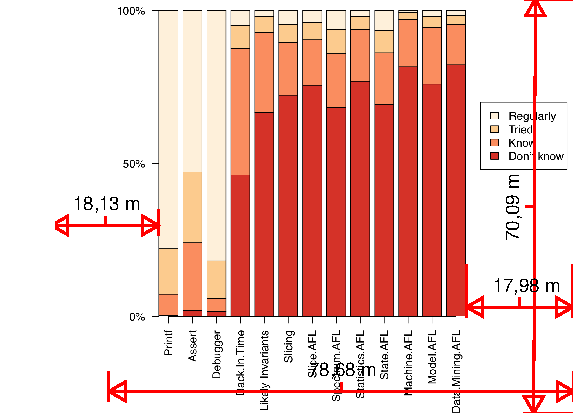
\includegraphics[width=.8\linewidth]{img/tool-usage}
\caption{Answers to "Which debugging tools do you know?"~\cite{perscheid17:studying_the_advancement}.}
\label{fig:tool-usage}
\end{figure*}

\section{Do We Need More Debugging Tools?}

Comparing figures \ref{fig:debugging-timeline} and \ref{fig:tool-usage}, we can see that a disconnect between the state of the art in research and the application of debugging in practice began to occur around the 1980ies.
Today, we can find a large number of debugging tools, techniques, and prototypes that are very good at what they do, but not widely used by developers.

Consistently with debugging studies, talking to professional software developers we learned that many developers are not even aware that advanced debugging techniques (\ie anything beyond symbolic debugging) exist and may even be available for the programming languages they use.
When developers told us they had heard of an advanced debugging methodology before, they knew not whether respective tools were available for their programming language and were surprised when told that such tools were available.
%If developers know of an advanced debugging tool, they often cited a lack of documentation as the main reason for not using it.
%While locating a software fault, developers don't want to divert attention to learning a new tool.
%\todo{performance issues}

Apparently, developers will not search for new debugging tools while locating a software fault.
But even when better tools are available, switching tools causes an interruption in the thought process that can slow down developers significantly~\cite{altmann14:momentary_interruptions_can_derail}.
Integrating debugging tools directly in the IDE and ensuring they fit the developers' workflow reduces this barrier by improving the accessibility of tools~\cite{wasserman90:tool_integration_in_software, stenning87:on_the_role}.
However, developers still need to know how to use these tools.
Here, it is not enough to expect developers to spend time learning the functionality and features, as "nobody reads documentation"~\cite{rettig91:nobody_reads_documentation} and formal education in debugging is rare~\cite{perscheid17:studying_the_advancement, ballou08:improving_software_quality}.
Instead, the user experience has to be designed such that features can be discovered when needed, without overwhelming the user with too much information and too many options~\cite{brockmann90:the_why_where}.

Thus, instead of only proposing new methods to better locate and repair software faults, 
researchers need to consider the developer as a user of the method, too.
Furthermore, choosing a specific use-case or "niche", instead of developing general purpose debugging tools,
allows to create tools more useful and accessible, at least for the chosen use-case, and further reduce the barriers of entry~\cite{wotawa17:panel_discussion}.

%In the survey by Perscheid et al., developers rated IDE integration and installation less
%important for the adaptation of new debugging tools than ease of use and documentation.
%However, considering 1.2 and what developers told us, it seems that not knowing
%that tools exist is the greatest obstacle.

%These findings show that it is not enough for debugging research to propose new methods
%to better find and repair software faults
%Based on these findings we conclude that 
%Thus, it is not enough for debugging research to propose new methods to better find and fix bugs.
%Having a wide selection of options to tackle a problem is only an advantage if users know how to select the best option and can apply it correctly.
%Thus, researches need to consider the developer as a user of the tool or method, too.
%Debugging tools need to seamlessly integrate into the developer's workflow and tool chain, and allow the exploration of features instead of requiring a formal training of the user.

\section{Millions of Lines of Code to Run a Business}

In our work, we focus on developers of enterprise applications as our target group;
\ie while our results may be useful for developers of other types of applications as well, we consider only problems of developers in this particular field for our design and evaluation.

Enterprise applications, \ie software that supports or automates business pro-\linebreak{}cesses~\cite{fowler02:patterns_of_enterprise_application}, are often large and complex.
\Ac{erp} systems, for instance, have to manage large amounts of business data, interact with many other computer systems, and adhere to complex legal requirements~\cite{linthicum00:enterprise_application_integration}.
SAP’s business suite already consists of several million lines of code~\cite{mallach15:information_systems_what_every}. 
On top of this, optional modules and custom extension are added to provide all required functionality.

The size alone already makes it difficult to locate bugs efficiently.
There is much more code that developers need to understand and the average length of infection chains, the distance between observed failure and responsible code fault, grows accordingly.
On top of that, there is technical complexity that slows down fault localization efforts.

%\begin{figure}
%\centering
%\begin{minipage}{.56\textwidth}
  %\centering
  %\includegraphics[height=50mm]{img/s4hana}
  %\captionof{figure}[High-level architecture of S/4 HANA]{High-level architecture of an S/4 HANA installation with XS applications~\cite{sap17:setup_of_sap_fiori}\linebreak}
  %\label{fig:s4hana}
%\end{minipage}~~~%
%\begin{minipage}{.42\textwidth}
  %\centering
  %\includegraphics[height=50mm]{img/xsa}
  %\captionof{figure}[Architecture of the SAP HANA XS Advanced framework]{Architecture of the SAP HANA XS Advanced framework~\cite{subatin17:xs_advanced_for_not}}
  %\label{fig:xsa}
%\end{minipage}
%\end{figure}

\begin{figure}
  \centering
  \includegraphics[width=.7\textwidth]{img/s4hana}
  \caption[High-level architecture of S/4 HANA]{High-level architecture of an S/4 HANA installation with XS applications~\cite{sap17:setup_of_sap_fiori}}
  \label{fig:s4hana}
\end{figure}


\Cref{fig:s4hana} shows the high-level architecture of SAP's business suite "S/4 HANA" from a technical perspective. 
On the left, the two major components, the ABAP front-end and back-end servers, contain the majority of business logic.
User clients, shown at the top, interact with the system using a browser with HTML5 support or the SAP GUI.
At the bottom of the stack, the SAP HANA database stores and manages application data.
On the right, additional reporting and analytics applications run in the SAP HANA Extended application Services (XS) Advanced framework.
Each product of the business suite, such as the ERP or CRM system, can add modules to all components in this architecture.

\begin{figure}
  \centering
  \includegraphics[width=.5\textwidth]{img/xsa}
  \captionof{figure}[Architecture of the SAP HANA XS Advanced framework]{Architecture of the SAP HANA XS Advanced framework~\cite{subatin17:xs_advanced_for_not}}
  \label{fig:xsa}
\end{figure}

The architecture of the XS Advanced framework is shown in more detail in~\cref{fig:xsa}.
Again, we find a browser-based client with a JavaScript UI library at the top and the SAP HANA database at the bottom.
In the center, the XS Advanced application framework supports server-side applications written in JavaScript, Java, or C++.
The dashed lines indicate communication across execution environment boundaries.

%Complex software systems often consist of multiple interoperating components written in different programming languages and running in different environments.
Both architectures match the three-tier application pattern~\cite{fowler02:patterns_of_enterprise_application}:
A database layer handles persistence and data-intensive computations.
On top, the application layer implements most of the business process logic and acts as a gateway to the client.
In the client, the user interface layer provides a rich user experience and sends requests to the application back-end to trigger actions and obtain data.
Because of the heterogeneous technologies, each layer typically comes with its own tool set and no tool can be used to work on all layers at once.

%Bugs can occur in any layer but often manifest themselves as failures in the user interface.
%Thus, developers first have to guess in which layer the error originated before choosing the appropriate debugging tool for that layer.
%If the guess turns out to be wrong, developers have to switch tools and context before continuing the bug hunt.
%Locating bugs in the interaction between two layers becomes even more difficult, as developers may have to switch tools several times to understand the fault.

%As these diagrams illustrate, enterprise applications consist of multiple interoperating components written in different programming languages and running in different environments.
Software faults can occur in any component but often manifest themselves as failures in the user interface.
Thus, developers first have to guess in which component the error originated before choosing the appropriate debugging tool for that component.
If the guess turns out to be wrong, developers have to switch tools and context before continuing the bug hunt.

To demonstrate the difficulty of localizing faults in complex systems, \cref{fig:worstcase} shows an example that is close to a worst-case scenario based on the S/4 HANA architecture.
A fault in the ABAP Front-End server causes corrupted data to be passed down into the database.
Later, the data is retrieved by an XSA application and causes a failure in the client.
Dashed lines indicate boundaries of execution environments.
As can be seen, to follow the infection chain from the failure to the fault, developers would have to switch debugging tools six times.

\begin{figure*}[t]
\centering
\includegraphics[width=.9\linewidth]{img/worstcase}
\caption{Bad case of an infection chain crossing several runtime environments}
\label{fig:worstcase}
\end{figure*}

Locating faults in the interaction between two components becomes even more difficult, as developers may have to switch tools back and forth repeatedly to understand the fault.
To efficiently debug a multi-tier application, developers would need a single debugger that is not only capable of debugging each layer but also aware of the interaction between layers at a meaningful level of abstraction.
Additionally, the debugger needs to provide help
navigating the large amounts of code that a long infection chain passes through
and consider database tables as part of the program state.

%Furthermore, the debugger needs to include the database
%Finally, to help developers handle the complexity and size of an enterprise application, the debugger should provide analysis features that integrate in the debugging process, instead of interrupting it.

%Looking back at the history of debugging, we find that innovations in debugging were usually quickly adopted when they occurred alongside changes in how software was developed.
%Recent trends in database technology and software engineering practices fundamentally affect how enterprise applications will be developed in the future~\cite{plattner15:the_in-memory_revolution_how}.
%We looked at these trends to identify specific problems today's developers have to face when debugging their code that can not be adequately solved with existing tools. 

\section{Our Approach} %(Research Questions \& Contributions) Our Approach

%\newcommand{\RQ}[1]{\paragraph{\emph{#1}}}
\newcommand{\RQ}[1]{\subsection*{\textsl{#1}}}

The overarching motivation of this work is to reduce the time and effort needed to locate faults in multi-tier enterprise applications.
In the past decades, many advanced debugging techniques have been developed that are not widely used in practice for various reasons.
By adapting  debugging techniques specifically to the needs of enterprise application developers,
while also keeping an eye on overhead and usability, we expect to increase their usefulness and accessibility such that they are more appealing in practice.

Looking back at the history of debugging, we find that innovations in debugging were usually quickly adopted when they occurred alongside changes in how software was developed.
Recent trends in database technology and software engineering practices fundamentally affect how enterprise applications will be developed in the future~\cite{plattner15:the_in-memory_revolution_how}.
%We looked at these trends to identify specific problems today's developers have to face when debugging their code that can not be adequately solved with existing tools. 
%Looking at these trends, 
Confirming previous studies~\cite{eisenstadt97:my_hairiest_bug_war, perscheid17:studying_the_advancement}, our research (cf. \cref{sec:enterprise_applications}\todo{cite}) has shown that much hardship for developers debugging enterprise applications is caused by long infection chains that cross boundaries of execution environments.
From this insight, we derived our research question:
%Thus, we defined the following research question:

\medskip
\noindent
\emph{How can advanced debugging techniques be adapted to reduce the time and effort needed to track long infection chains across sub-system boundaries in multi-tier enterprise applications?}
%\blockquote{How can advanced debugging techniques be adapted to reduce the time and effort needed to track long infection chains across sub-system boundaries in multi-tier enterprise applications?}
\medskip

\noindent
Omniscient debugging, for instance, can significantly improve fault localization, but imposes a large overhead on run-time and memory cost.
Developers will be reluctant to use tools if the required costs outweigh the expected benefits.
However, the longer the infection chain, the more of a difference \acfp{odb} can make.
We identified three areas were current omniscient debugging tools do not meet the needs of developers of enterprise applications.

%\RQ{Contribution 1: A method for the faster navigation of long infection chains}

%When developers debug a program, they are typically not just "browsing" the execution, but rather searching for something specific.
%In particular, when tracking an infection chain the most common operation is to find the origin of a potentially erroneous value.
%In large and complex systems, infection chains tend to be very long as well.
%Thus, if a debugging tool can increase the speed with which developers can track infection chains, the overall time needed to locate a bug can be reduced.

%The debugger's vast knowledge about the execution can be used for dynamic analyzes.

\emph{Interactive Dynamic Slicing} is a new debugging workflow that addresses the need to track long infection chains through large amounts of code.
Generally, there are two major approaches to fault localization: manual debugging, \eg using \acp{odb}, and \acf{afl}.
\Acp{odb} make it easier to freely navigate a program execution, but offer no specific help for tracking down relevant code locations.
Many \ac{afl} techniques, on the other hand, can identify code locations likely related to a failure, but do not provide a way to verify this relation.
Furthermore, the accuracy of \ac{afl} diminishes over longer distances.
Combining both approaches, however, keeps their advantages while reducing their drawbacks.

The execution history available to the \ac{odb} can be used to quickly compute dynamic slices to help developers to identify relevant code.
With Interactive Dynamic Slicing, while debugging the dynamic slice, at any point developers can add or adjust the slicing criteria.
A new slicing algorithm allows for incremental configuration of a slice. 
This way changes are applied instantly, without interrupting the debug session. 
A new UI component, the \emph{Slice Navigator}, provides a unique view on the execution by combining relevant information from both the \ac{odb} and the slicing subsystem.


%\RQ{Contribution 2: Back-in-time debugging on the database layer}

\emph{TARDISP} is a debugger that brings back-in-time debugging down to the database layer.
Enterprise applications are very data-driven.
Developers need direct access to the database not only to understand the context and evaluate the correctness of an operation, but the data itself, with erroneous or unexpected values, can be the source of software failures.
In such cases, developers must not only identify the responsible data records, but also determine how they found their way into the database.

With back-in-time debuggers, developers can explore what happened before observable failures by following infection chains back to their root causes. 
While there are several such debuggers for object-oriented programming languages, we do not know of any back-in-time capabilities at the database-level.
Thus, if failures are caused by components that interact with the database, developers have difficulties in understanding their unexpected behavior.

We developed an approach for bringing back-in-time debugging down to the database.
Our \emph{TARDISP} debugger allows developers to step queries backwards and inspecting the database at previous and arbitrary points in time. 
With the help of an SQL extension, developers can express queries covering a period of execution time within a debugging session and handle large amounts of data with low overhead on performance and memory. 
The entire approach has been evaluated within a development project at SAP and shows promising results with respect to the gathered developer feedback.

%\RQ{Contribution 3: Seamless omniscient debugging across the layers of a 3-tier architecture}

The \emph{TARDISP full stack debugger} extends TARDISP to aggregate traces from multiple concurrent executions into one continuous debug session.
Even with back-in-time debugging available in every layer of the software stack, developers still have to switch tools when following an infection chain along requests between sub-systems.
Switching tools imposes a significant cognitive overhead on developers and can break their productive flow.

Assuming back-in-time debugging capabilities for each application tier, 
we introduce hierarchical step numbering based on synchronization points between components to create a partial ordering of instructions in all concurrent executions.
A visualization in the front-end shows developers which UI element is affected by which back-end operation, providing them with a top-down summary of the execution.
A second visualization is shown in the debugger and helps developers to navigate the application flow.

\section{Contributions} 
summarize again \\ \\
1) Interactive dynamic slicing combines AFL and ODB \\
- new slicing algorithm \\
- Slice navigator UI\\
\\
2) BiT down to the database\\
- model for re-executing queries\\
- SQL extension\\
\\
3) system debugger\\
- unified model\\
- top-down view\\


%% improve debugging;  
%This challenge will be approached from two directions.
%First, recent debugging innovations need to be made more available in practice.
%It is not enough to simply make more features available in debugging tools, the features need to be conveniently accessible and the cost of learning a new feature must not be too high at any point in time.
%Second, debugging tools need to move along with recent technology trends.
%Developers need better support debugging applications that handle large amounts of data and are composed of sub-systems with heterogeneous technology stacks.
%From this, we defined three research questions.
%
%% mtiier verbessern ; verfolgen
%
%\RQ{Research Question 1: How can debuggers help developers to navigate a program when following a long infection chain?}
%
%When developers debug a program, they are typically not just "browsing" the execution, but rather searching for something specific.
%In particular, when tracking an infection chain the most common operation is to find the origin of a potentially erroneous value.
%In large and complex systems, infection chains tend to be very long as well.
%Thus, if a debugging tool can increase the speed with which developers can track infection chains, the overall time needed to locate a bug can be reduced.
%
%There are two major approaches to fault localization: manual debugging, \eg using \acfp{odb}, and \acf{afl}.
%\Acp{odb} make it easier to freely navigate a program execution, but offer no specific help for tracking down relevant code locations.
%Many \ac{afl} techniques, on the other hand, can identify code locations likely related to a failure, but do not provide a way to verify this relation.
%Furthermore, the accuracy of \ac{afl} diminishes over longer distances.
%By combining both approaches, however, we believe we can keep their advantage while reducing their drawbacks.
%%The debugger's vast knowledge about the execution can be used for dynamic analyzes.
%
%We developed \emph{interactive dynamic slicing}, a new debugging workflow that combines omniscient debugging and dynamic slicing. 
%The execution history available to the \ac{odb} can be used to quickly compute dynamic slices to help developers to identify relevant code.
%While debugging the dynamic slice, at any point developers can add or adjust the slicing criteria.
%A new slicing algorithm allows for incremental configuration of a slice. 
%This way changes are applied instantly, without interrupting the debug session. 
%A new UI component, the \emph{Slice Navigator}, provides a unique view on the execution by combining relevant information from both the \ac{odb} and the slicing subsystem.
%
%\RQ{Research Question 2: How can programs handling large amounts of data be debugged and analyzed efficiently?}
%
%Enterprise applications are very data-driven.
%Developers need direct access to the database not only to understand the context and evaluate the correctness of an operation, but the data itself, with erroneous or unexpected values, can be the source of software failures.
%In such cases, developers must not only identify the responsible data records, but also determine how they found their way into the database.
%
%With back-in-time debuggers, developers can explore what happened before observable failures by following infection chains back to their root causes. 
%While there are several such debuggers for object-oriented programming languages, we do not know of any back-in-time capabilities at the database-level.
%Thus, if failures are caused by components that interact with the database, developers have difficulties in understanding their unexpected behavior.
%
%We developed an approach for bringing back-in-time debugging down to the database.
%Our \emph{TARDISP} debugger allows developers to step queries backwards and inspecting the database at previous and arbitrary points in time. 
%With the help of a SQL extension, developers can express queries covering a period of execution time within a debugging session and handle large amounts of data with low overhead on performance and memory. 
%The entire approach has been evaluated within a development project at SAP and shows promising results with respect to the gathered developer feedback.
%
%\RQ{Research Question 3: How can developers debug complex systems without being impeded by control-flow crossing sub-system boundaries?}
%
%Even with back-in-time debugging available in every layer of the software stack, developers still have to switch tools when following an infection chain along requests between sub-systems.
%Switching tools imposes a significant cognitive overhead on developers and can break their productive flow.
%
%Assuming back-in-time debugging capabilities for each application tier, 
%we extended TARDISP to aggregate traces from multiple concurrent executions into one continuous debug session.
%We introduce hierarchical step numbering based on synchronization points between components to create a partial ordering of instructions in all concurrent executions.
%A visualization in the front-end shows developers which UI element is affected by which back-end operation, providing them with a top-down summary of the execution.
%A second visualization is shown in the debugger and helps developers to navigate the application flow.

\section{Outline}

The remainder of this thesis is structured as follows:

\Cref{sec:debugging_in_ea} provides background on our work.
We describe the process which developers typically use to locate faults with a debugger, how it changes with back-in-time debugging.
Furthermore, we outline the typical components of an enterprise application and how debugging is affected by recent changes in technology.

In \cref{sec:ids}, we present interactive dynamic slicing, a new debugging workflow that combines omniscient debugging with dynamic slicing.
A new slicing algorithm allows developers to incrementally change a slice. 
The Slice Navigator, a novel GUI component, combines access to the debugger and the slicer in a single view.
With a user study, we show that our approach allows for more efficient fault localization, even for developers that are not yet familiar with the tools.

\Cref{sec:db_odb} focuses on back-in-time debugging in the database.
We present an approach to efficiently trace and replay the execution of programs handling large amounts of data,
an SQL extension allowing developers to query past data and filter for changes between points in time,
and a prototype implementation of our approach.
%a prototype implementation to database developers and gathered valuable feedback that confirms the usefulness of our approach.

In \cref{sec:stack_odb}, we describe a model for hierarchical omniscient debugging of concurrent executions and propose visualizations that can help developers to navigate control flow in a multi-tier application.

In \cref{sec:relatedwork}, we discuss related work in the area of back-in-time debugging, slicing, and analysis of enterprise applications.

\Cref{sec:conclusion} suggests areas for improvement and future work and concludes.


%How can debugging be improved to reduce the time needed to find a bug?
%\\- How can developers efficiently navigate a program execution?
%\\- How can the debugger help to identify relevant code?
%\\- How can programs handling large amounts of data be debugged and analyzed efficiently?
%
%A better way to track failure causes
%\\- Improved existing program analysis technique 
%\\- Seamless integration into debugging workflow
%\\- Allows more efficient debugging by increasing focus, providing more relevant information, and reducing tool-related interruptions
%
%Efficient omniscient debugging in the database
%\\- Fully featured ODB with little overhead on performance and memory
%\\- Query past database states
%\\- Query changes in the database



\chapter{Debugging in Enterprise Applications}
\label{sec:debugging_in_ea}

Debugging is the process of finding and resolving defects in a computer program~\cite{araki91:a_general_framework}.
Efficient debugging requires a good understanding of the program and the ability to distinguish correct and incorrect program behavior, i.e., some external knowledge about the program's requirements.
Accordingly, debugging tools can assist developers by identifying relevant code locations for review, by analyzing and visualizing program behavior, and by suggesting fixes.
% knowledge: I. Vessey. Expertise in Debugging Computer Programs: A Process Analysis

In this chapter, we present approaches to debugging that built the foundation of our work and discuss specific challenges in the context of enterprise applications.

%\section{How To Debug a Program}
\section{The Scientific Approach to Fault Localization}

% Experienced developers are able to locate defects up to three times faster and add fewer new failures than novices
% J. Gould. Some Psychological Evidence on How People Debug Computer Programs.

% novices add more errors
% L. Gugerty and G. Olson. Comprehension Differences in Debugging by Skilled and Novice Programmers.
The starting point for a debugging task is a known program failure, an observed deviation from correct program behavior.
Developers with only little debugging experience often debug with an incomplete understanding of the program, modifying the code until the failure can no longer be reproduced~\cite{gugerty86:comprehension_differences_in_debugging}.
These modifications may be based on educated guesses but otherwise follow no particular strategy.
While this trial-and-error based approach usually works for simple bugs, it has several critical drawbacks.

Firstly, there is a significant risk of introducing additional bugs into the system~\cite{gugerty86:comprehension_differences_in_debugging,yin11:how_do_fixes_become}, especially when developers fail to consider the side-effects of their changes or incorrectly undo wrong guesses.
Most importantly, however, this method can not be used to approach more complex bugs effectively.
Some bugs need fixes at multiple code locations or have a large conceptual distance between the observed failure and the defect in the code.
In such cases, developers risk entirely missing the root cause of the problem~\cite{gu10:has_the_bug_really},
\ie while they may succeed in fixing one of its symptoms, the actual bug remains in the system.
To overcome these problems, developers need a more structured approach to debugging, one that separates localizing and fixing the fault.

Experienced developers often follow a process that is similar to the scientific method~\cite{araki91:a_general_framework}.
\Cref{fig:scientifiy-method} shows the process as a flow chart.
First, developers formulate a hypothesis explaining the failure; then, they attempt to verify the hypothesis through an experiment. 
\begin{figure*}[t]
\centering
\includegraphics[width=.4\linewidth]{img/workflow-scientific-method}
\caption{The scientific approach to fault localization.}
\label{fig:scientifiy-method}
% R. Metzger. Debugging by Thinking - A Multidisciplinary approach.
\end{figure*}
If the experiment does not confirm the hypothesis, developers must improve their understanding of the program in order to form a better one.
If the experiment confirms the hypothesis, however, it has not necessarily revealed the root cause of the failure.
Sometimes, the hypothesis is to vague and the problem needs to be narrowed down further.
In other cases, the experiment revealed that the erroneous behavior of one component was caused by incorrect input of another component, in which case a new failure cause becomes the focus of investigation.
Either way, developers repeat the hypothesis-experiment cycle until they identify the root cause and can begin the repair.

\section{Back-in-Time and Omniscient Debugging}
\label{sec:omni-debugging}

Very often, defective code does not cause the program to fail immediately.
Instead, it creates an error in the program state that propagates, in accordance to the garbage-in-garbage-out principle, until it yields to a failure in a different part of the application.
This sequence of erroneous states is also called the infection chain~\cite{zeller09:why_programs_fail}.
Developers tasked to locate the defect have to follow the infection chain backwards through execution time.

%Tools can support the fault localization process 

\begin{figure*}[th]
\centering
\includegraphics[width=.9\linewidth]{img/workflow-traditional}
\caption{Following an infection chain with a debugger.}
\label{fig:workflow-traditional}
\end{figure*}

\Cref{fig:workflow-traditional} shows how developers track an infection chain with a debugger.
Beginning at the failure, developers follow the infection chain backwards through execution time.
Each step consists of forming a hypothesis and confirming it by inspecting the relevant code location with a debugger. \todo{explain image in more detail}
Following this method, developers will continually get closer to the root cause of the bug.
If developers have not enough knowledge of the program to identify relevant code locations for the next step, the debugger can also be used to explore the program execution to find suspicious locations.
Thus, debuggers can help developers with both tasks in the scientific debugging approach.

However, debuggers have one major limitation: they do not allow developers to go back.
Developers track the infection chain backwards through time.
As \cref{fig:workflow-traditional} shows, to move backwards a new debug session has to be started at every step.
Likewise, when using a debugger to explore an execution, developers might accidentally step over a method instead of stepping into it, either because they did not expect relevant behavior to occur inside that method or simply because of pressing the wrong button.
In both cases, the debug session has to be restarted to get back in time.

Restarting the debugger is usually an easy task, and getting to the desired point in the execution can be as simple as setting a breakpoint at the respective location.
Alas, often getting to the right point is more cumbersome.
For instance, it may happen that the breakpoint is hit multiple times.
In this case developers have to either resume the execution repeatedly until the right point in time is reached, or set a breakpoint at a different location that is hit less often and manually step from there.
Either way demands high concentration from the developer as making a mistake means having to start all over again.
In other cases manual interaction with the program is required to set up the program state in which the error will occur.
This, too, has to be repeated with every restart of the debug session.
Thus, while restarting the debugger is in the best case a simple operation that imposes only a small delay on the developer, it often is a complex task that requires careful attention.
This attention is then drawn away from solving the actual problem.

\begin{figure*}[t]
\centering
\includegraphics[width=.9\linewidth]{img/workflow-odb}
\caption{Following an infection chain with a back-in-time debugger.}
\label{fig:workflow-odb}
\end{figure*}

%%---------
\emph{Back-in-time debuggers} seek to remedy this problem by allowing developers to step backwards.
This all but removes the need to restart the debugger.
\Cref{fig:workflow-odb} shows how developers track the infection chain with a back-in-time debugger.
Instead of restarting at every step, developers move back and forth along the data-flow, thereby reducing the time needed for each hypothesis-confirmation cycle.

Different approaches exist to realize back-in-time debugging.
Recording lost state allows the debugger to roll back changes by reversing each instruction~\cite{feldman88:igor_a_system,cook02:reverse_execution_of_java,lieberman95:zstep_95_a_reversible}.
By creating regular snapshots of the entire program state, the debugger can go back faster over longer distances in time~\cite{boothe00:efficient_algorithms_for_bidirectional,tolmach93:a_debugger_for_standard}.
% TODO: about IO
%%----
Many different strategies can be used to realize back-in-time capabilities in a debugger.
These strategies come with different trade-offs between overhead and usefulness.

With a regular debugger, the only way to go back in time is to restart the execution.
Tools can be used to automate this approach, but some manual effort is often required to get to a specific point in time.
The clumsiness of this approach is what motivated research in back-in-time debuggers in the first place.
On top of that, this approach only works when the execution is deterministic and does not depend on external factors, such as resources or timing.
Some debuggers even allow to restart executions at the method level.
This greatly improves the usability when developers want to re-examine the program flow, but as state changes are not reverted executing a method multiple times can have unintended side-effects.

To improve determinism when re-executing code, snapshot-based debuggers record the program memory at regular intervals~\cite{feldman88:igor_a_system, boothe00:efficient_algorithms_for_bidirectional}.
%%----

A special kind of back-in-time debugger, called \emph{omniscient debugger}, keeps a record of all state changes in the execution history~\cite{lewis03:debugging_backwards_in_time}.
This not only allows developers to step backwards in time, it also opens the possibility to run structured queries on the history of program states.
For example, an omniscient debugger can easily list all invocations of a method or show a history of all field accesses in an object.
Such information can be very helpful for developers trying to understand a program and is not easily obtainable through other means.

Recording the entire execution history also allows the debugger to run \emph{post-mortem}, i.e., it simulates an active debug session while the actual program has already terminated.
This way, developers can not only restart the debugger later without having to re-run the program, but they can do so on a different machine or even share the recording with coworkers.
\todo{about memory usage}


%\subsection{Slicing}
\section{The Evolution of Slicing Algorithms}
\label{sec:evolution_of_slicing}

A different way how tools can support the debugging process is by helping to form hypotheses about the failure.
Better hypotheses reduce the number of iterations needed in the hypothesis-confirmation cycle and thereby shorten the time needed to locate a bug.
While developers first need to improve their understanding of the program in order to form better hypotheses, a tool can quickly analyze large parts of a program or program execution and suggest likely causes for a fault.
This approach is called \emph{automatic fault localization} and many techniques to locate suspicious code have been developed~\cite{wong16:a_survey_on_software}.
In our work, we build on one of these techniques, called "slicing".

Research has shown that developers also break programs down into pieces of code that are related by data flow~\cite{weiser82:programmers_use_slices_when}.
Such "slices" are often not contiguous and can contain code from many different parts of an application, increasing the navigation overhead for developers trying to understand the program.
Here, tools can help to identify related statements, saving time and reducing the mental overhead for developers.

In 1981, Weiser introduced slicing as a technique helping developers to find related code for a given question~\cite{weiser81:program_slicing}.
According to Weiser, a slice is a subset of a program that, when executed, yields the same state trajectory with respect to given slicing criteria as the original program would have.
The slicing criteria are pairs of variables and code locations.
An important property of the resulting slice is that it must be executable.
This allows the slice to be compiled and inspected with a debugger.

Weiser proposed an algorithm for computing static slices, i.e., slices that are correct for every possible input of the program.
Static slices often are very large, especially for complex applications, and many sophisticated methods have been developed to reduce the size of static slices~\cite{ottenstein84:the_program_dependence_graph, lyle93:program_slicing_in, hoffner95:evaluation_and_comparison}.

In 1988, Korel and Laski proposed to compute slices that are valid only for one specific program input~\cite{korel88:dynamic_program_slicing}.
Such dynamic slices can be much smaller than static slices because the slicer has to consider only one concrete execution path~\cite{venkatesh95:experimental_results_from_dynamic, hoffner95:evaluation_and_comparison}.
However, to achieve this we must add the program input to the slicing algorithm's parameters.

Shortly after Korel and Laski, Agrawal and Horgan independently also introduced dynamic slices~\cite{agrawal90:dynamic_program_slicing}.
Agrawal and Horgan used an approach based on execution traces that allowed to remove more statements than previous approaches, but the resulting slices were not always executable.
Thus, they defined "accurate slices" as slices that contain all statements relevant for computing the state trajectory for the slicing criteria, but are not necessarily compilable or executable.
Agrawal \etal\ also presented SPYDER, a tool that allows debugging non-executable slices by superimposing the slice on an execution of the full program~\cite{agrawal93:debugging_with_dynamic_slicing}.

\begin{figure*}[t]
\centering
\includegraphics[width=.75\linewidth]{img/slice_usefulness}
\caption{As a slice becomes smaller its usefulness increases, until the fault itself is removed.}
\label{fig:slice_usefulness}
\end{figure*}

Subsequent work focused on increasing the precision of accurate slices, for example in the presence of pointers~\cite{atkinson02:program_slicing_using_dynamic, agrawal91:dynamic_slicing_in}.
In 2003, Zhang \etal\ presented three algorithms to efficiently compute "precise slices", i.e., slices that are "accurate" but contain little to no statements that could be removed~\cite{zhang03:precise_dynamic_slicing_algorithms}.
Like many other authors, Zhang \etal\ argued that producing small slices is essential if slicing is to be "an attractive option" for developers.
However, Korel argued that slicing too aggressively can also be dangerous, as
for program debugging the challenge is not necessarily to minimize the size of the slice at any cost but rather to minimize the size of the slice without the elimination of faulty program statements~\cite{korel98:dynamic_program_slicing_methods}.
\Cref{fig:slice_usefulness} illustrates the problem as a graph.
A slice that contains all the code is just as useful as having access to the code itself.
When more and more code is removed, the usefulness grows as less code has to be investigated by developers.
But when slicing becomes so aggressive that the code developers are actually looking for is removed, too, 
the slice's usefulness drops drastically.
Slicing algorithms therefore try to err on the safe side and are generally cautious when estimating whether code can be removed.

Between executable and "accurate" slicing algorithms, the former are the more conservative.
Their difference can be demonstrated with a small example.
In the code shown in \cref{lst:sliceAccurate}, line 9 is only executed during the second iteration of the loop.
Therefore, when choosing ´ratio´ in line 9 as a slicing criterion, "accurate" slicing algorithms can remove the assignment of the first array item in line 3.
This will reduce the size of the slice, as the call to ´complexComputation1´ is removed, but when the remaining code is executed, a division by zero will occur during the first iteration in line 7.
Korel argued that the correctness of a slicing algorithm can not be objectively determined if it is allowed to produce slices where the program fails~\cite{korel98:dynamic_program_slicing_methods}.
Without proven correctness, one risks falling off \cref{fig:slice_usefulness}'s usefulness cliff.

\begin{lstlisting}[float,caption={Code example for accurate slices.},stepnumber=2,numberfirstline=false,label=lst:sliceAccurate,language=Java]
	void main() {
			float[] data = new float[2];
			data[0] = complexComputation1(); // returns 0.5
			data[1] = complexComputation2(); // returns 5
			for (float f: data) {
					f = adjustValue(f);
					float ratio = 2 / f;
					if (ratio < 1) {
							System.out.println(ratio); // expected 0.2, got 0.4
					}
			}
	}

	float adjustValue(float value) {
			if (false && moreConditions()) { // bug in this line
					return value * 2;
			}
			return value;
	}
\end{lstlisting}

However, algorithms for both executable and "accurate" slices are allowed to remove the call to ´adjustValue´ in line 6 and can therefore hide the actual bug.
In general, bugs caused by wrongly skipped or missing code are difficult to locate with slicing.
Wang \etal\ addressed this problem by developing an algorithm to find "relevant" slices, slices including code that could have changed the state trajectory but was not executed~\cite{wang08:dynamic_slicing_on_java}.
Likewise, Ko \etal\ developed Whyline, a slicing-based tool allowing developers to ask "Why?" and, more importantly, "Why not?" questions~\cite{ko08:debugging_reinvented_asking}.

The usefulness of a slice depends not only on which code remains included, but also on what the developer wants to achieve.
While a slice may be suitable for solving one problem, for another problem the necessary code might have been removed.
By considering developers with a debugging problem as end users of a slicing tool, we can carry the trend of carefully reducing slice sizes to its logical conclusion: we define a "most useful slice" as exactly the subset of statements of a program that developers need to see in order to answer the question they are currently investigating.
Such a slice is not necessarily executable, "accurate", "precise", or "relevant", according to the established definitions, but rather captures the optimal combination of these conflicting properties.

Some approaches attempt to provide better slices by making assumptions about developers' information needs~\cite{sridharan07:thin_slicing}.
We argue that additional user input is necessary to provide better slices without risking to remove to much code.
Thus, to compute a "most useful" slice, we would have to add the developers' research question and current state of mind to a slicing algorithm's input.
This leaves us with two problems.
Firstly, we need to find a method to formalize a developer's entire state of mind, and secondly, we need to a way for developers to specify this data easily and correctly.
%While it may not be possible to achieve perfect "most useful" slices in one attempt, we can look into ways to approximate

%Alas, we cannot present a solution for either of these problems.
%\todo{
%However, as a step towards the goal of "most useful" slices, we developed a slicing algorithm that allows developers to easily get arbitrarily close to the smallest slice they need.}

\section{Additional Challenges in Enterprise Applications}
\label{sec:enterprise_applications}

\tmpStart
To better understand the development of modern business software, we interviewed five software developers from SAP, a German software corporation developing enterprise software to manage business operations.
From these developers, we gained insights on the development of four different projects:
\begin{enumerate}
	\item A software for liquidity risk management that analyzes the cash-flow of financial institutes to assess their liquidity,
	\item A customer analytics software to understand customer behavior based on collected data, which allows, for example, to identify particularly profitable customers or customers that plan to leave the company (e.g., clients of a bank who cancel all their standing orders),
	\item A product for predictive analytics that allows to estimate the probabilities for certain customer behaviors, such as switching distributors or suppliers. The analyses' results are integrated in a customer relationship management (CRM) system and recommend opportunities for salespeople, and
	\item The point-of-sales (POS) explorer, a dashboard that computes various key performance indicators (KPIs) on the revenue and profits of products based on retail data.
\end{enumerate}
%
All applications are designed to work on real-time data generated by respective transactional systems and were developed with an industry partner who provided requirements.

\subsection{Changing Characteristics in 3-tier Applications}

The design of all applications was based on the 3-tier architecture pattern, which divides an application into three layers~\cite{eckerson95:three_tier_clientserver_architecture}.
The \emph{presentation tier} displays information and receives input from the user,
the \emph{application tier} contains the application's business logic, and
the \emph{data tier} encapsulates data access and persistence.
The presentation tier is the application's front-end and runs on the client, while the application and data tier constitute the back-end and run on the server.

In traditional 3-tier applications, most of the code is implemented in the application layer.
For example, templates allow the application server to render web pages that can be displayed by a browser on the client.
When a dedicated client application is needed, keeping it small and simple reduces the overhead of maintaining and updating a large number of installations.
Either way, the client is little more than a terminal.

On the data side, object-relational mappers (ORMs) allow developers to implement data processing logic directly in the application.
This makes applications independent from specific database products and avoids introducing additional programming languages into the project.
Because application servers can be scaled more easily than databases, this also reduces the database bottleneck that can occur in applications with many users.

Many application frameworks, such as J2EE and Ruby on Rails, follow this philosophy and many tools have been developed to support development and maintenance in such ecosystems.
However, as we found in our interviews, the usefulness of many of such tools is decreasing as technologies and requirements change in the development of modern business applications.
For illustration, \cref{fig:3tier-changes} compares the architectures of exemplary classical and modern 3-tier applications.

\begin{figure*}[t]
\centering
\includegraphics[width=.9\linewidth]{img/3tier-changes}
\caption{As a slice becomes smaller its usefulness increases, until the fault itself is removed.}
\label{fig:3tier-changes}
\end{figure*}

HTML 5 and JavaScript allow developers to build responsive and dynamic interfaces, which are increasingly expected by users.
Via HTTP and fast connections, megabytes of client code can be updated with every request so there is no longer a need to keep the client code minimal.
JavaScript-based GUI libraries eliminate the need for server-side templates as the entire GUI can be built in the client and data is dynamically loaded via AJAX requests.

With big-data becoming more important for many companies, it is no longer feasible to handle all data operations in the application layer.
Even transactional systems contain a large fraction of analytical operations~\cite{krueger10:a_case_for_online} and high-performance databases can handle such queries faster than application-level code~\cite{plattner09:a_common_database_approach}.
Even for transactional operations, the usefulness of ORMs is doubted as they can introduce other organizational and architectural problems~\cite{neward06:the_vietnam_of_computer}.

All developers reported that their projects followed these new architecture patterns.
To achieve sufficiently low response times, data is stored in \emph{SAP HANA}, a high-performance in-memory relational database.
The application layers run in \emph{SAP HANA Extended Application Services}, an application and web server environment on top of the database.
In each project, the front-end is implement in \emph{SAPUI5}, a JavaScript GUI library based on jQuery.

For the fourth project, the POS explorer, we were given full access to the code base.
At the time of the interview, the whole application had 11 thousand lines of code, libraries excluded.
55\% of the code (i.e., about 6000 lines) was client-side JavaScript, of which about 12\% (725 lines) was data querying code.
The application layer consisted of 2000 lines (18\%) of server-side JavaScript (similar to node.js), while the database layer contained 3000 lines (27\%) of stored procedure code.
Data schema definitions are not included in the line counts, as the data is defined and provided by other applications.
% client/js					2397
% client/fragment		3750
% client/view				 133
% client -- query		 600 // client 6280 -- 6000
% app/xsjs*					2250 //  -- 2000
% db/procedure			2991 // -- 3000
% // 11521

Standards like \emph{OData}~\cite{chappell11:introducing_odata} allow clients to submit arbitrary queries to the database, entirely eliminating the need for a middle layer.
It should be noted that this setup is different from the classical 2-tier architecture, where a trusted client has full access to the database.
OData still maintains security concerns such as authentication, authorization, and visibility of data, which was previously a responsibility of the application tier.

For one of the projects, the developer reported that they have no application layer code at all.
The application, he estimated, consisted of 90\% client-side JavaScript, of which one-third was OData client code, and 5\% OData service configuration which passed requests to stored procedures that constituted the remaining 5\% of the project.

In conclusion, due to increased complexity of interactions between the different layers it is no longer sufficient to be able to debug each layer on its own.
Instead, tools are needed that help developers to debug and understand the application as a whole.

\subsection{Debugging 3-tier Business Applications}

All developers reported that changes in software development processes affected the way how bugs are handled.
In the past, large applications had separate development teams for front-end, business logic, and data management.
If a team found that a bug was not caused in their respective domain, the responsibility was passed on to the next team.

Agile development methodologies, such as Scrum or Extreme Programming, discourage dividing teams by technology layer.
Instead, requirements and, if necessary, sub-teams are now grouped around feature sets.
Thus, while there still may be developers who are specialized on one of the application tiers, every developer is expected to be able to work on and to debug every layer.
This increases the need for making debugging tools for each layer easily available to all developers.

The existence of bugs is typically discovered by observing unexpected data in the user interface.
Then, developers use their browser's development tools to examine the request with which the data was obtained.
In most cases, the response data is passed unchanged to the GUI components and the incorrect data can be tracked directly back to the response.
Here, the first uncertainties occur as it is often not obvious whether the request was submitted with incorrect arguments or whether the error is on the server-side.

If developers decide to continue to the application code, they determine which server function is called, connect a debugger to the application server, set a breakpoint, and re-submit the failing request.
Then they use the debugger to understand how the request is processed.

If no fault can be found, they now need to determine if the results returned by database queries are correct.
For queries that include complex views or stored procedures, this is not an easy task.
Furthermore, if the query was composed at runtime, developers also need to determine the actual query string and which arguments were used.
After that, they can use the tools provided by the database client to analyze the query and verify the result.

Using these methods, developers move up and down the stack until they find the root cause of the bug.
Generally, all developers reported that they preferred to work with a top-down approach, i.e., they try to first understand the interaction between the layers before starting a debugger to narrow down possible locations for the bug as early as possible.
However, while the developer tools of browsers were reported to be somewhat useful for this task, no such tools exist to understand the interaction between application and data tier at a glance.

Overall, frequent switches between tools were reported to be a major distraction when trying to focus on the program flow.
Often, multiple monitors were used to allow developers to access all tools more quickly, but all developers wished for better integration between tools.
\tmpEnd

%\section{Requirements for an Enterprise Application Debugger}
%\label{sec:requirements}
%
%Based on what we learned about
%
%
%Requirements
%- Iterative approach
%- Identify related statements \cite{ko07:information_needs_in_collocated}
%- support short-term memory \cite{fry97:programming_on_an_already}
%- reduce problem size



%Finding bugs in complex code is a demanding task for developers and many tools and techniques have been developed to support this process.
%However, complex system architectures add another level of difficulty to fault localization.
%
%Server-based applications typically use a three-tier architecture.
%The database layer is used to persist the application's domain model.
%The user interface layer shows application data to the user and accepts user input.
%In between, the application layer contains most of the business logic which defines the application's workflows, how to handle user requests, and how to collect and present requested data.
%
%When most code resides in the application layer, so do most bugs and the well-known debugging tools can be used to locate them.
%However, in more recent years, the classic three-tier architecture changed in multiple ways.\todo{source}
%
%\subsection{Database Layer}
%
%The amounts of data to be handled by server-based applications are always increasing.
%Recently, big data has become a very important topic for many enterprises.
%To guarantee optimal performance on large data sets, more and more data handling code has to move closer to data, into the database layer.\todo{source}
%
%tbd: describe UI technologies
%
%\subsection{User-Interface Layer}
%
%Better web browsers, HTML 5, and Java Script replaced the terminal application.
%It is now easier to manage client code as updates are automatically requested via HTTP.
%This way, more business logic could move into the UI layer to provide a better user experience.\todo{source}
%
%tbd: describe UI technologies
%
%\subsection{Application Layer}
%
%Remaining AppLayer: request mapping, security
%
%Java, Rails, Node.js
%
%skip applayer with ODATA and user-management in database
%
%\subsection{Debugging the Stack}
%
%Both modern browsers and databases have debugging capabilities that are useful to locate bugs within their respective layers.
%Alas, not every bug can be tracked down to a single code location. 
%Sometimes, it is a combination of mismatching assumptions in different code locations that compose the fault \todo{source}.
%In a complex system, these locations need not reside in a single component, but can be scattered across all layers.
%Likewise, the infection chain that connects the observed failure with the fault in the code can cross several system boundaries.
%
%In both cases, no single debugging tool is sufficient to locate the bug, as each debugger can only be used to debug its respective system.
%The resulting tool and context switches impose a mental overhead that distracts developers from the actual problem.
%
%The problem is further amplified with service-oriented architecture (SOA), and micro-services in particular.
%To achieve better scalability and faster life-cycle management, applications are broken down into many independent systems, each with their own database.
%While the resulting modularization can help to limit the consequences of software failures to smaller sub-systems, the difficulty of locating cross-system bugs increases further.
%
%%The debugger is one of the most important tools of a software developer. 
%%It allows to observe and inspect a program’s execution and can be used for many purposes, such as bug detection and code comprehension. 
%%Workflow
%%\\- failure observed
%%\\- error in state- > find the code
%%\\- either GIGO, then repeat, or...
%%\\- fault in code
